\chapter{Extracellular conductivity}
\label{chap:Sigma}
\index{Conductivity}
%\tvnnote{Is the book about 'modelling extracellular potentials', or more broadly 'extracellular potentials'? If it is the latter, maybe we should say "key concept" instead of "key parameter/variable"?}
A key \tvntxt{concept} in volume conductor (VC) theory is the extracellular conductivity, $\sigma_t$. In most applications of VC theory, $\sigma_t$ is assumed to be a constant, and its value is normally taken from some experimental measurement. Estimates can vary greatly between different recordings, but common values are between 0.2 and 0.5~S/m.
Throughout the previous section, we assumed that $\sigma_t$ was homogeneous, isotropic and frequency independent. In this chapter we discuss these assumptions. In addition, we discuss some experimental and theoretical estimates of  $\sigma_t$. Before doing so, however, we introduce the continuous, porous medium approximation in some detail, to show what $\sigma_t$ actually represents.

\begin{figure}[!ht]
\begin{center}
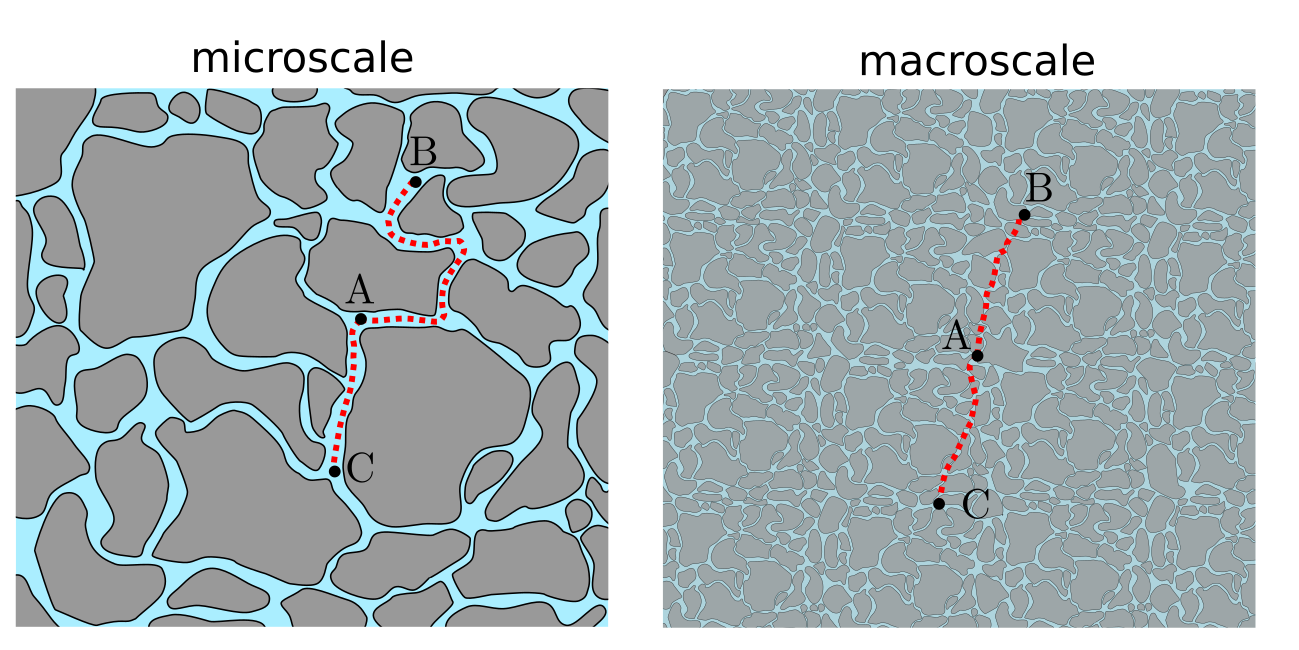
\includegraphics[width=0.6\textwidth]{Figures/Sigma/ecs.png}
\end{center}
\caption[]{\textbf{Illustration of a piece of brain tissue.} Extracellular space (light blue) occupies only about a fraction $\alpha$ of the total tissue volume, and has a highly tortuous structure. The tortuosity, $\lambda$, is defined as the ratio between the shortest pathway between two points in space and the euclidian distance between these two points, and accounts for the fact that ions traveling through the medium do not travel in straight lines, but need to take detours around cellular obstacles.
(A) $\alpha$ and $\lambda$ vary on the microscopic scale. For example, the shortest path (red dotted curve) between locations $r_0$ and $r_1$ is more tortuous than the path between locations $r_0$ and $r_2$. (B) On a larger spatial scale, local inhomogeneities average out, and the tissue can be treated as homogeneous. Typical tissue averages for $\alpha$ and $\lambda$ are 0.2 and 1.6, respectively \cite**{Nicholson1998,Sykova2008}. \ghnote{Omform figur i traad m/ figtekst}
\tvnnote{Legg paa panelmarker, A,B}
}
\label{fig:Sigma:ECS}
\end{figure}

%%%%%%%%%%%%%%%%%%%%%%%%%%%%%%%%
\section{\blue{Continuous, porous medium approximation}}
\label{sec:Sigma:continuous}
\index{Continuous medium}
\index{Porous medium}

%%%%%%%%%%%%%%%%%%%%%%%%%%%%%%%%
When presenting the theory for modeling single neurons (Chapter \ref{chap:Neuron}), we may have given the impression that they are solitary creatures living in a vast extracellular space with long distances to their nearest cell neighbors\tvnnote{Could mention that this mental image also stems from the early staining procedures (Cajal, Golgi, Nansen :-)), where only a small fraction of neurons were actually stained. If all had been stained, it would have been pure black}. \tvntxt{If this had been true, the extracellular conductivity would in practice have been that of saline.} This is far from the truth. A cross-section of a piece of brain tissue shows that it is densely packed with neurons and glial cells (\fref{fig:Sigma:ECS}), and that the extracellular space (colored light blue in the figure) occupies only about 20\% of the the total tissue volume.
\tvntxt{Currents moving through the extracellular medium
are typically assumed to move mostly through the extracellular space, while the cells are effectively non-conducting bodies \cite**{Robinson1968,Nunez2006}.}
\tvntxt{From this, we can already make a first rough estimate of the extracellular conductivity: The extracellular saline has a conductivity of about 1.5~\si{\siemens / \metre}, but only occupies about 20\% of the space, meaning that we might expect the extracellular conductivity to be on the order of 1.5~\si{\siemens / \metre} $\cdot$ 0.2 = 0.3~\si{\siemens / \metre}. This value fits perfectly well with the values typically measured in experiments, although the calculation itself vastly underestimates the complex electrical properties of neural tissue.}

The extracellular space has a highly tortuous \index{Tortuosity} geometry, with an average \tvntxt{extracellular distance between cell membranes of only} about 40-60~nm \cite**{Sykova2008}.
At the micrometer scale, the conductivity \index{Conductivity} $\sigma$ in brain tissue is \tvntxt{therefore} highly non-homogeneous and anisotropic. For example, the conductivity in a certain spatial direction will depend on whether there locally is a free extracellular passage in that direction (high conductivity), or whether this passage is blocked by a nearby membrane (low conductivity) (\fref{fig:Sigma:ECS}{\bf A}). 
%Likewise, also the electric potential $\phi$ will vary greatly over tiny distances, depending on the proximity to neural membranes, especially when approaching the nanometer thick Debye-layers building up the membrane charge \cite**{Pods2013}\tvnnote{Kanskje denne setningen hoerer mer hjemme i VC eller Basics?}.
%When we study extracellular potentials, we are typically not interested in these microscopic variations in $\sigma$ and $\phi$, but rather in the values of these entities when averaged over some spatial volume. Electrodes used to record extracellular potentials typically have sizes ranging from 5 $\mu$m to 125 $\mu$m in diameter \cite**{Viswam2019}, which is larger than the typical diameter of a dendrite ($\sim$ 1 $\mu$m). In practice, the electrodes therefore perform such an averaging, and include contributions from several nearby neurons \tvnnote{Remove last half of sentence? Seems like a different issue to me}. \tvnnote{Tok bort dette, da jeg tenker vi dekker dette et annet sted?}
\tvntxt{At a slightly larger spatial scale, of tens or hundreds of micrometers, it is however reasonable to assume that these micrometer scale inhomogeneities average out (\fref{fig:Sigma:ECS}{\bf B}), and that the brain tissue can be treated as a continuous, porous medium \cite**{Nicholson1981,Gratiy2017}. 
This assumption is further motivation by the lack of any alternative, since we can not in experimental settings know the exact microstructure of the brain.} The VC theory presented in the previous chapter was based on the continuous, porous medium approximation, and thus describes the extracellular dynamics on a spatial resolution larger than at least a few micrometers.

A continuous, porous medium is defined by two key parameters \cite**{Nicholson1981}. The first parameter, $\alpha$, is the fraction of the tissue volume that is extracellular space. The second parameter is $\lambda$, the tortuousity of the extracellular medium \cite**{Nicholson1981}. It is defined as the ratio between the shortest \tvntxt{extracellular} pathway between two points in space and the euclidian distance between these two points, and accounts for the fact that ions traveling through the medium do not travel in straight lines, but need to take detours around cellular obstacles. The parameters $\alpha$ and $\lambda$ can be measured experimentally. Typical values are $\alpha = 0.2$ and $\lambda = 1.6$, although these values vary between brain regions and even locally due to cellular swelling or shrinkage \cite**{Nicholson1998,Sykova2008}.
\tvnnote{Mention that $\alpha$ also varies considerably with brain state, for example with sleep? If I remember correctly, Nagelhus et al (inlcuding Klas) tried to measure brain conductivity to assess brain-state or something like that?}

The continuous, porous medium approximation has implications for how we interpret the various concepts and variables that we use to compute extracellular potentials. In particular, it is important for how we understand the conductivity of the tissue medium. In this chapter, we shall compare three different conductivity measures, and we list them here for clarity and later reference:

\begin{itemize}

\item $\sigma_{saline}$ (S/m) is the conductivity of the saline solution that fills up the extracellular space, and is determined by the ion concentrations in the saline solution (see Section \ref{sec:Sigma:concentrationbased}). Since the brain fortunately contains more than just the extracellular solution, $\sigma_{saline}$ only applies microscopically in the small gaps between neurons, and is not the conductivity of brain tissue as a whole.
\tvntxt{The value of $\sigma_{saline}$ is typically measured to be about 1.5~S/m \cite**{Logothetis2007,Martinsen2008,Miceli2017}.}
\item $\sigma_{e}$ (S/m) is the conductivity of the \textit{extracellular medium} \index{Extracellular medium}, as experienced at a macroscopic (coarse-grained) scale by a current traveling exclusively trough the extracellular part of brain tissue. Importantly, this current does not pass through a 3D volume filled exclusively with the \textit{extracellular solution}, but (i) is confined to move only through a fraction $\alpha$ of the total medium volume, and (ii) must take detours around neural and glial obstacles, as reflected through the tortuousity $\lambda$ \cite**{Nicholson1998,Nunez2006}. The macroscopic $\sigma_{e}$ should theoretically be a factor $\alpha/\lambda^2$ lower than the microscopic $\sigma_{saline}$ (see Section \ref{sec:Sigma:concentrationbased}).

\item $\sigma_t$ (S/m) is the macroscopic (coarse-grained) conductivity of the brain tissue, and is the conductivity as experienced by a macroscopic (coarse-grained) current traveling through the tissue. It is $\sigma_t$ (S/m) that one normally measures experimentally, and it is $\sigma_t$ that is the relevant for use in VC theory. If currents through brain tissue were indeed confined to stay exclusively in the extracellular part of it, $\sigma_t$ should be identical to $\sigma_e$. If currents through brain tissue goes through intracellular pathways in addition to the extracellular ones, we would expect
$\sigma_t$ to be greater than $\sigma_e$ \cite**{Okada1994}.

\end{itemize}




%%%%%%%%%%%%%%%%%%%%%%%%%%%%%%%%
\section{\blue{Anisotropic conductivity}}
\label{sec:Sigma:Anisotropic}
\index{Conductivity!Anisotropic}

%%%%%%%%%%%%%%%%%%%%%%%%%%%%%%%%
\tvntxt{Neural tissue typically has clearly anisotropic geometrical properties, for example, 
the very numerous cortical pyramidal cells tend to be geometrically aligned along the depth direction of cortex.
It makes intuitive sense that this anisotropy could also be reflected in the conductivity, so that the conductivity in the depth direction of cortex could differ from the conductivity  in the perpendicular directions.
In \fref{chap:VC}, we assumed that the tissue conductivity $\sigma_t$ was isotropic, i.e., the same in all the spatial directions, however
this is not always true. For example, in cortex it has been found that the conductivity is about 1.5-fold higher in the depth direction, i.e., for currents running in parallel to the axis of pyramidal cell dendrites \cite**{Goto2010}. The cerebellum has an even more pronounced anisotropic geometrical structure, and the conductivity in the depth direction has been found to be about 3-fold higher than in the perpendicular directions for the anuran cerebellum \cite**{nicholson1975}. Finally, a pronounced anisotropy in the conductivity is typically observed in white matter, because the axons are typically oriented in similar directions by the formation of fiber bundles \cite**{Nicholson1965,Logothetis2007,Bangera2010}. This anisotropy in the conductivity of white matter can in certain cases be as strong as a 10-fold increase in conductivity along the fiber bundle \cite**{Nicholson1965,Bangera2010}.
}

However, the overall effect of the anisotropy on extracellular potentials, at least in cortex, often appears to be quite weak \cite**{Logothetis2007,Ness2015,Miceli2017}, and the approximation that $\sigma_t$ is isotropic often gives good predictions of the potential. See~\fref{fig:Sigma:anisotropy_effect} for an example where a 1.5-fold increase in the conductivity along the axis of the apical dendrite \cite**{Goto2010}, only causes a slightly more squeezed shape of the extracellular potential than the isotropic case \cite**{Ness2015,Miceli2017}. Since extracellular potentials are rather insensitive to modest anisotropies, by far the most common approach is to assume that the extracellular conductivity, at least in cortex, is isotropic.

\begin{figure}[!ht]
\begin{center}
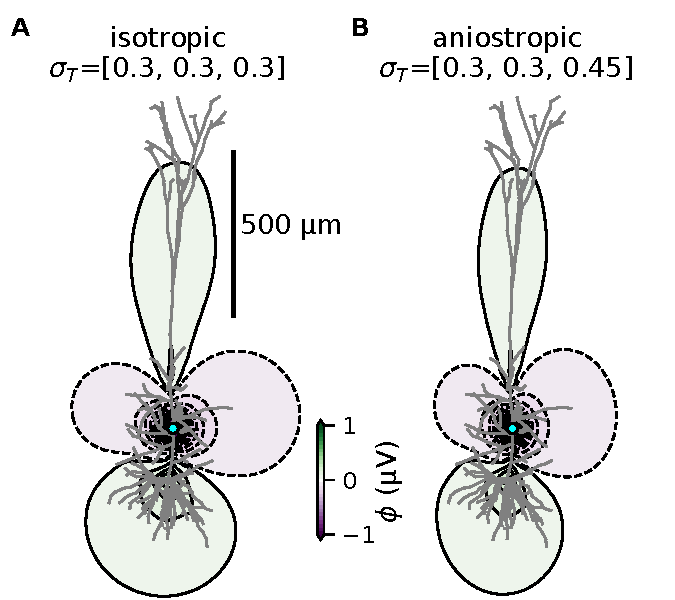
\includegraphics[width=0.6\textwidth]{Figures/Sigma/fig_anisotropy_effect.pdf}
\end{center}
\caption[]{\textbf{Effect of modest anisotropy.}
Extracellular potential at a snapshot in time following a single excitatory synaptic input (location marked by cyan dot) to a rat cortical layer 5 pyramidal neuron \cite**{Hay2011}.
The extracellular potential is shown for the time step corresponding to the maximum observed absolute value for the extracellular potential, and it is calculated from the same neural simulation, at the same time with either an isotropic extracellular medium ({\bf A}) or with an anisotropic extracellular medium, with a 50\% higher
conductivity along the axis of the apical dendrite ({\bf B}). The calculation with anisotropic conductivity was done with \fref{eq:Sigma:Panisos}.
}
\label{fig:Sigma:anisotropy_effect}
\end{figure}

%\tvnnote{Give example already here of where this is particularly relevant?: White matter, Cerebellum, and also mention 50\% increase in cortex, from Goto.}
When deemed necessary, it is relatively straightforward to expand the VC theory to the case of an anistotropic $\sigma_t$. In this case, $\sigma_t$ will no longer be a scalar, but instead a tensor with the three components $\sigma_{tx}$, $\sigma_{ty}$ and $\sigma_{tz}$.
If we use the point source approximation (\fref{eq:VC:pointsources}), the extracellular potential surrounding a set of point current sources $I_k$ is given by \cite**{nicholson1975,Parasnis1986}:

\begin{equation}
\phi(x,y,z) = \sum_k \frac{I_k}{4\pi\sqrt{\sigma_{ty}\sigma_{tz} (x-x_k)^2 + \sigma_{tx}\sigma_{tz} (y-y_k)^2 + \sigma_{tx}\sigma_{ty} (z-z_k)^2}}.
\label{eq:Sigma:Panisos}
\end{equation}
If we use the CSD-description of the sources (eq.~\ref{VC:eq:csds}), the corresponding expression is:
\begin{equation}
\phi(x,y,z) = \iiint_V \frac{C(x,y,z)}{4\pi\sqrt{\sigma_{ty}\sigma_{tz} (x-x_k)^2 + \sigma_{tx}\sigma_{tz} (y-y_k)^2 + \sigma_{tx}\sigma_{ty} (z-z_k)^2}} \, dV.
\label{eq:Sigma:Canisos}
\end{equation}
\tvnnote{Should we derive this in an appendix? It seems it is quite hard to find a derivation of this in the literature, but I managed to find one eventually. (Parasnis1986)}

%\ghnote{Trenger vi en presisering her? Hva betyr det at effekten er lav? Jeg tenker at 50 prosent stoerre sigma burde gi 50 prosent stoerre amplituder, og det er vel ikke en svak effekt? Mener vi at spenningen i en utvalgt retning er relativt upaavirket av anisotropi i andre retninger enn den utvalgte?}
%\tvnnote{La til figur. Vi ble overasket i Ness et al. (2015), over at det nesten ikke var noe synlig effect, hverken naar det var simulert med FEM eller med punktkilde-formlene. Forskjellen kan kanskje kvantifiseres bedre, men er det noe vits?}



%%%%%%%%%%%%%%%%%%%%%%%%%%%%%%%%
\section{\blue{Nonhomogeneous conductivity}}
\label{sec:Sigma:nonhomo}
\index{Conductivity!Nonhomogeneous}
\tvnnote{In- or non-homogeneous?}
In \fref{chap:VC}, we assumed that the extracellular conductivity $\sigma_t$ was homogeneous, i.e., the same everywhere. Clearly, this assumption does not hold on the micrometer scale, where neural tissue is highly non-homogeneous \cite**{Nicholson1998}, see \fref{fig:Sigma:ECS}.
On a very large spatial scale, for example at the scale of whole brains, it is again clear that the tissue is non-homogeneous, since the brains, even for large primates, are not infinite in size.
However, on a mesoscopic spatial scale the microscale inhomogeneities tend to average out (cf. the continuous medium approximation), while the boundaries to other tissue types or materials are often sufficiently distant to have a negligible effect on extracellular potentials. In such cases, for example within a given brain region such as cortex, a homogeneous conductivity appears to be a reasonable approximation \cite**{nicholson1975,Okada1994,Logothetis2007,Goto2010,Ness2015}.

There are however still many scenarios where an infinite homogeneous medium is not a reasonable assumption,
typically because of boundaries between neural tissue and other tissue types or materials.
%For example, for electric potentials measured close to the surface of the brain, the transition from neural tissue  (like for ECoG measurements, see also \ref{chap:ECoG}),
%The situation is different when signals are recorded very far from their sources. It is then likely that they on their journey have experienced a $\sigma_t$ that varied on a macroscopic scale \tvnnote{Er det egentlig riktig aa snakke om "reisen" til et potensial? }.
%For example, electroencephalography (EEG) signals recorded outside of the head are strongly affected by the presence of the brain tissue, cerebrospinal fluid (CSF), skull and scalp, which are very different media with different electrical  conductivities.
When the extracellular medium is non-homogeneous, there is no general analytical formula available (like eqs. \ref{VC:eq:csds}, \ref{eq:Sigma:Panisos} or \ref{eq:Sigma:Canisos}) that link the extracellular potentials to the underlying current sources. In principle, one can however always solve eq. \ref{VC:eq:CSD2} for arbitrarily complex geometries with varying conductivities using numerical methods, like the Finite Element Method (FEM) \cite**{Logg2012}.
This approach has for example been used to model electroencephalography (EEG) signals recorded outside of the head, because these potentials are not only affected by the conductivity of brain tissue, but also by the presence of the cerebrospinal fluid (CSF), skull and scalp, which have widely different conductivities. This is covered in more detail in \fref{chap:EEG}.
Substantial inhomogeneities can also be introduced into neural tissue through the presence of big electrode shanks, as briefly discussed in \fref{sec:VC:elec_shafts}.
%For examples of neuroscience applications using this approach, see \cite**{Moffitt2005,Frey2009,Joucla2012,Haufe2015,Ness2015,Buccino2019b,Obien2019}.

\subsection{Planar boundaries: The cortical surface and {\it in vitro} slice recordings}
For some simple and highly symmetric cases of inhomogeneous volume conductors, analytical solutions can be found for calculating extracellular potentials from the underlying current sources.
An important example of this is (approximately) planar boundaries between different tissue-types or different materials. In such cases, we can use the Method of Images (MoI)\index{Method of Images} from electrostatics \cite**{Jackson1998} to account for the effect of a planar boundary on the extracellular potential from current sources \cite**{Gold2006,Pettersen2006,Nunez2006,Ness2015,Obien2019}. This is done by introducing virtual current sources on the opposite side of the boundary with the same distance to the boundary as the original point current sources, and with the amplitudes scaled by \cite**{Nunez2006,Ness2015},
\begin{equation}
W = \frac{\sigma_1 - \sigma_2}{\sigma_1 + \sigma_2}.
\label{Sigma:eq:MoI_scaling}
\end{equation}
Here, $\sigma_1$ is the conductivity of the region containing the real current sources, and $\sigma_2$ is the conductivity of the region at the other side of the boundary containing the virtual sources.
For example, before inserting recording electrodes into the brain the cortical surface will typically be exposed, and materials of widely different conductivity can be used to cover the cortical surface.
To account for the effect of the different conductivity of cortex and the cover material, the point source equation
(\ref{eq:VC:pointsource2}) must be modified \cite**{Nicholson1971,Pettersen2006},
\begin{equation}
\phi({\bf r}) = \frac{I_k}{4\pi \sigma_t |{\bf r-r_k}|} + \frac{\sigma_t - \sigma_{\rm cover}}{\sigma_t + \sigma_{\rm cover}} \frac{I_k}{4\pi \sigma_t |{\bf r-r_k'}|},
\label{eq:Sigma:MoI}
\end{equation}
where ${\bf r}_k'$ is the location of the virtual current source, mirrored across the cortical surface.
Note that the equation on this form is
only valid within the region with the real source, while other formulas apply outside of this region \cite**{Nunez2006}.
The material at the cortical surface can substantially affect potentials measured near the cortical surface, as illustrated in \fref{fig:Sigma:cortical_surface_effect}.
In particular, notice from \fref{eq:Sigma:MoI} the special case of a measurement performed at the planar boundary to a non-conducting region, so that $|{\bf r-r_k}|=|{\bf r-r_k'}|$, and $\sigma_{\rm cover}=0$. In this case, the measured potential will be exactly a factor of two larger than for an infinite homogeneous medium.

\begin{figure}[!ht]
\begin{center}
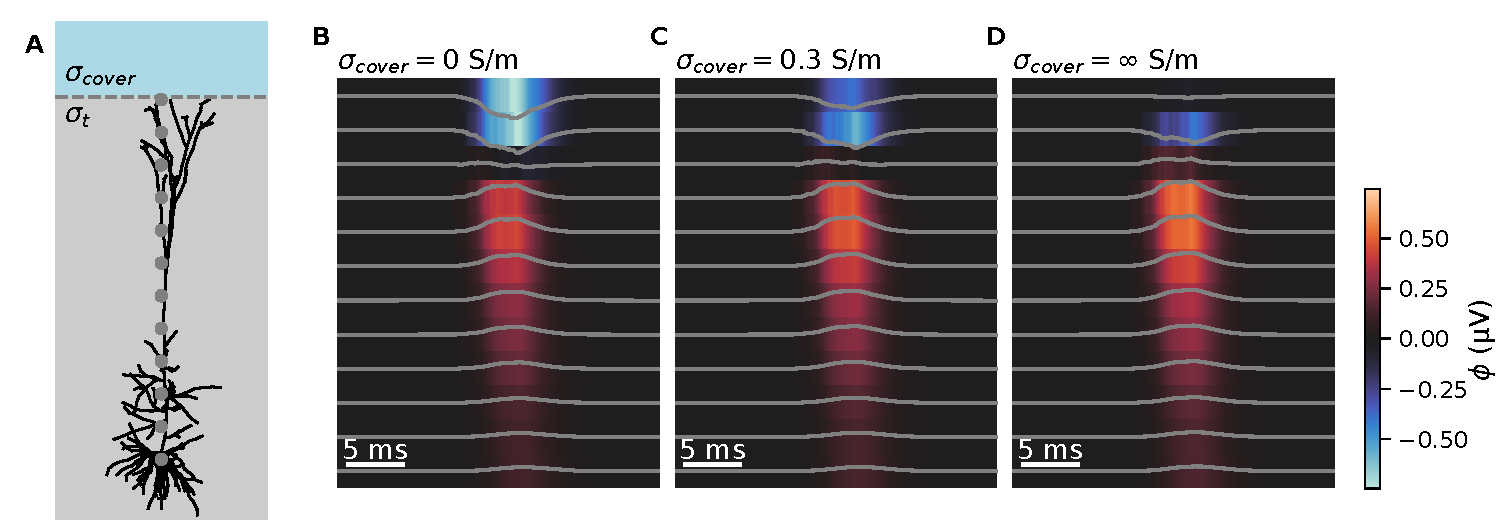
\includegraphics[width=1\textwidth]{Figures/Sigma/fig_cortical_surface_effect_MoI.pdf}
\end{center}
\caption[]{\textbf{Effect of inhomogeneity of cortical surface}
{\bf A:} Simulation set-up. A rat cortical layer 5 pyramidal cell \cite**{Hay2011} receives a wave of excitatory synaptic input to the upper apical dendrite (top 200~$\mu$m). The conductivity of cortical tissue is $\sigma_t$=0.3~S/m, while different conductivities of the region above cortex is tested.
{\bf B:} The cover is an insulator, $\sigma_{\rm cover}$ = 0.0~S/m, like a non-conducting mineral oil or air.
{\bf C:} The cover has the same conductivity as tissue, $\sigma_{\rm cover}$ = 0.3~S/m, corresponding 	to an infinite homogeneous volume conductor.
{\bf D:} The cover is highly conductive, $\sigma_{\rm cover}$ = $\infty$~S/m, like a metal plate.
See also \citeasnoun**{Pettersen2006}.
}
\label{fig:Sigma:cortical_surface_effect}
\end{figure}
%%%%%%%%%%%%%%%%%%%%%%%%%%%%%%%%

The same framework with MoI can also be used to model {\it in vitro} slice recordings, where a small slice of neural tissue is extracted from a brain and placed on a micro-electrode array (MEA), immersed in a saline bath. In this case, there are two planar boundaries, namely the lower boundary between the slice and the non-conducting MEA (glass) electrode plate, and the upper boundary between the slice and the saline bath, see \fref{fig:Sigma:MEA_illustration}.
The two boundaries instead of one gives rise to an infinite series of virtual current sources, which for the simplest case of the measurement being performed at the lower boundary to a non-conducting region, can be written like:
\begin{eqnarray}
\label{eq:Sigma:moi_PS}
\phi(x,y,0) & =  & \frac{2I}{4\pi \sigma_T} \bigg( \psi_{PS}(x,y,z')  \nonumber \\
& + & \sum_{n=1}^{\infty} W_{TS}^n\bigg[ \psi_{PS}(x,y,-z' + 2nh) + \psi_{PS}(x,y,-z' - 2nh) \bigg ]\bigg),
\end{eqnarray}
with 
\begin{equation}
\psi_{PS}(x,y,\tilde z) \equiv \left((x-x')^2 + (y-y')^2 + \tilde z^2)\right)^{-1/2}.
\end{equation}

For an example of this framework, for modelling spikes in {\it in vitro} slices, see \fref{fig:Spikes:MEA-spikes}, and for further details see \citeasnoun**{Ness2015}.
\begin{figure}[!ht]
\begin{center}
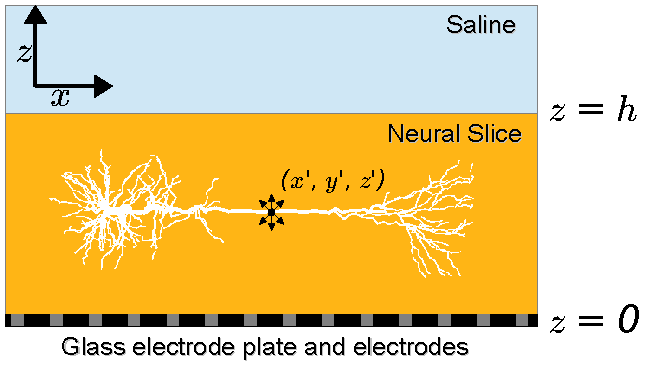
\includegraphics[width=0.4\textwidth]{Figures/Sigma/MEA_illustration.pdf}
\end{center}
\caption[]{\textbf{Illustration of MEA recording set-up.}
See also \citeasnoun**{Ness2015}.
}
\label{fig:Sigma:MEA_illustration}
\end{figure}
%%%%%%%%%%%%%%%%%%%%%%%%%%%%%%%%


\section{\red{TVN: Frequency dependence of the conductivity}}
\label{sec:Sigma:f-independent}
\index{Conductivity!Frequency dependence}
%\ghnote{GH: Skrev skisse til dette. Puttet figuren m/ sigma-maalinger inn her, da disse ser ut til aa primaert diskuteres opp mot eventuell frekvensavhengighet. Mulig vi burde ha med "eksperimentelle maalinger i kapittel-tittelen?}

%Regardless of the level of isotropy and homogeneity of a medium, its response to an imposed alternating current can depend on the frequency of the current. Then, the conductivity contains a resistive part, which is real and frequency independent, and an imaginary part that accounts for capacitive and inductive effects that are frequency dependent.
An important question for interpreting and modelling electric signals in neuroscience is whether the conductivity of neural tissue is frequency dependent. If a substantial frequency dependence is present, this would mean that the recorded signals are distorted as they propagate through the medium, and it would bias recordings towards certain parts of the frequency spectrum. In this subsection we will briefly cover the experimental measurements investigating this issue, as well as the theory needed to model such effects, should it be deemed necessary.

We have earlier stated that extracellular currents are typically assumed to move mostly through the extracellular saline solution, where the cells can basically be treated as non-conducting objects (\fref{sec:Sigma:continuous}). If this is true, we would expect the extracellular conductivity to be frequency-independent, since saline is known to be an ohmic medium \cite**{Martinsen2008}. 
A frequency dependence in the extracellular conductivity would not however in itself be surprising: As we have seen, the extracellular space is tightly packed with neurons, and because of the capacitive properties of their membranes, their membrane conductivity is highly frequency dependent (\fref{sec:Neuron:Cap}). Therefore, one could easily imagine that low-frequency extracellular currents are more confined to move resistively through the extracellular space, while
high-frequency extracellular currents could move both resistively through the extracellular space and capacitively through the cells. This would effectively introduce a higher conductivity for higher frequencies, thereby reducing the amplitude of high-frequency extracellular potentials (see \fref{eq:Sigma:pointsource_freq_dep}). This would for example imply that the low-frequency LFP signals are less attenuated than the high-frequency spikes. 
It has been suggested that "stability" of LFP and sensitivity of spikes to position is caused by this, and EEG has "only" low frequencies \cite**{Logothetis2007}, and 1/f power-laws in LFP.

Earlier investigations the frequency dependence of the extracellular conductivity (also called the impedance spectrum) reported little or no frequency dependence \cite**{Ranck1963,nicholson1975,Pfurtscheller1975}. However, a later study by \citeasnoun**{Gabriel1996} reported a substantial frequency dependence,
in particular below 100~\si{\hertz} (\fref{fig:Sigma:freq_dep}). 
More recent studies again seem to measure little or no frequency dependence of the extracellular conductivity \cite**{Logothetis2007,Elbohouty2013,Wagner2014,Dowrick2015,Miceli2017,Ranta2017,Avery2017}. 
It should be noted that these more recent studies typically consistently measure an increase of the conductivity of about 20-50\% from a few hertz to a hundreds or thousands of hertz, however, at least in some cases, a similar frequency dependence was also measured in saline, indicating that this frequency dependence at least partially originated in the recording equipment \cite**{Logothetis2007,Miceli2017}. 

\begin{figure}[!ht]
\begin{center}
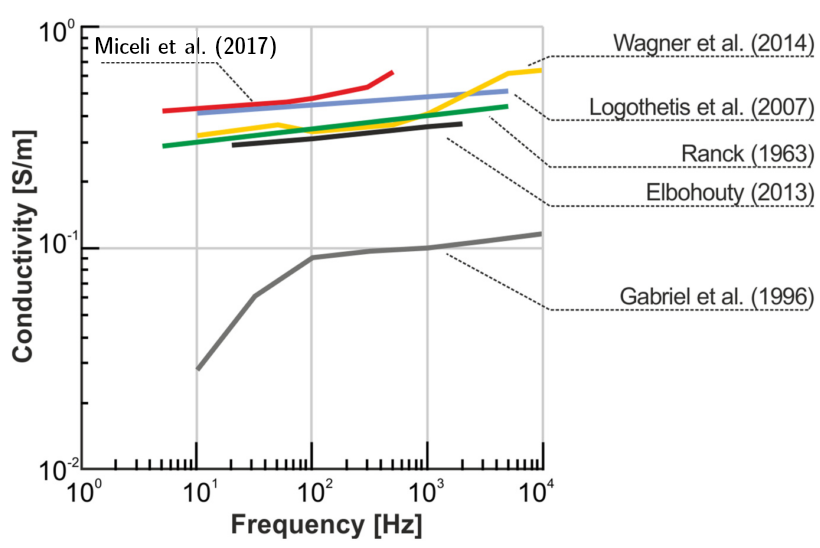
\includegraphics[width=0.6\textwidth]{Figures/Sigma/frequency_dependence.png}
\end{center}
\caption[]{\textbf{Literature review of reported conductivities in various species and experimental setups.}
Most studies seem to indicate a very weak frequency dependence of the extracellular conductivity\index{Conductivity}, which would have a negligible effect on measured extracellular potentials \cite**{Miceli2017}. The very low and strongly frequency dependent values measured by \cite**{Gabriel1996} represents an outlier, and although it has received substantial attention, it has to the best of our knowledge not been reproduced by any other study. For details about the data, see \cite**{Miceli2017}, and references therein \cite**{Ranck1963,Gabriel1996,Logothetis2007,Elbohouty2013,Wagner2014}.
}
\label{fig:Sigma:freq_dep}
\end{figure}

The study by \citeasnoun**{Gabriel1996} clearly stands out, as it is the only study to our knowledge to experimentally measure a strong frequency dependence below 100~\si{\hertz}. This study also reported a conductivity of only about 0.03~\si{\siemens/ \metre} at 10~\si{\hertz}, about an order of magnitude lower than the commonly reported values. This value seems surprisingly low, given that neural tissue contains a substantial fraction of highly conducting saline.
 The authors were however careful to note that the reported low-frequency values might be distorted by inadequate correction for electrode polarization (see also \fref{sec:VC:electrodes}). Further, a later study using the same recording equipment did not observe a similarly strong frequency-dependence, or similarly low conductivity values (\citeasnoun**{Wagner2014}; \fref{fig:Sigma:freq_dep}). Finally, their recording were done in bovine brains obtained from a slaughterhouse up to a couple of hours post-mortem \cite**{Gabriel1996}, which can potentially have resulted in suboptimal tissue preservation and cell swelling \cite**{Seoane2004}. 

Consequently, the extracellular
 it has been widely is to assume that it is not. 
However some indications: Gabriel, Bedard, Destexhe
(and somewhat controversial) 

In Section \ref{chap:VC:onlyohmic}) we argued that the extracellular displacement current is negligible, which means that the extracellular medium in itself (and thus $\sigma_e$) does not exhibit any capacitive effects. This alone does not rule out the possibility that the effective conductivity of the tissue medium ($\sigma_t$) includes capacitive effects, as currents traveling through it could interact with nearby capacitive neural membranes.

However, for the relevant frequencies in extracellular recordings (\fref{fig:Sigma:freq_dep}), the capacitive and inductive effects appear to be negligible compared to the resistive effects \cite**{Logothetis2007,Miceli2017,Ranta2017}. In most applications of VC theory, one therefore applies the assumption that the medium is Ohmic or resistive, meaning that the imaginary and frequency dependent part of the conductivity is zero. We note, however, that it is possible to expand the formalism to include a frequency dependent conductivity \cite**{Bedard2004,Tracey2011,Miceli2017}.


For a frequency-dependent conductivity, the point-source equation becomes \cite{Bossetti2008,Miceli2017}
\begin{equation}
\phi({\bf r}, \omega) = \frac{I}{4\pi (\sigma_t(\omega) + \vec j \omega \epsilon(\omega)) r},
\label{eq:Sigma:pointsource_freq_dep}
\end{equation}

%\tvnnote{Utledning tilsvarende Appendix B i Nunez?}
%\ghnote{Vet ikke helt.... Appendixet gir et greit bevis paa at kapasitive effekter i ECS er smaa. De foelger opp med et tilsvarende studium av membranen, men i det studiet er det membranen alene som er mediumet. Saa vidt jeg kan se faar vi ingen pekepinn paa hva membranens tilstedevaerelse gjoer for tissue-stroemmer....}


%\begin{figure}[!ht]
%\begin{center}
%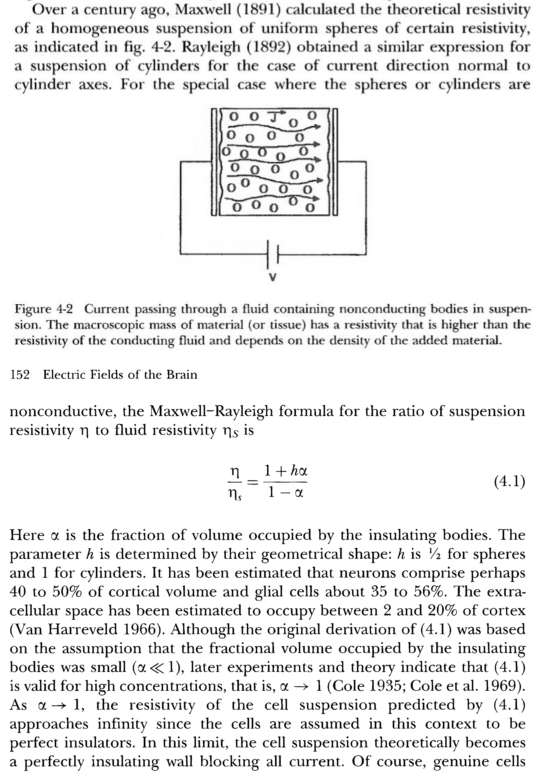
\includegraphics[width=0.6\textwidth]{Figures/Sigma/resistivity_maxwell.png}
%\end{center}
%\caption{\textbf{From Nunez} \tvnnote{Ta med noe slikt?}}
%\label{Sigma:fig:maxwell_resistivity}
%\end{figure}

\section{\red{TVN: Theoretical explorations....} }
\index{Conductivity!Theoretical estimates}

\ghnote{Dette var et punkt i den opprinnelige planen. Referenser: Meffin2012,
Tahayori2012, Meffin2014, Tahayori2014. Jeg vet ikke helt hva dette gaar i, men det gjoer sikkert Torbjorn og/eller Gaute?}


\section{\blue{GH: Theoretical estimate of the conductivity based on ion concentrations} }
\label{sec:Sigma:concentrationbased}
\index{Conductivity!Ion concentration dependence}

Extracellular current are mediated by the ions dissolved in the extracellular solution, and the conductivity of the extracellular medium if thus a function of thus depends on the ion concentrations, i.e., on the availability of free charge carriers \cite**{Grodzinsky2011}:

\begin{equation}
\sigma_{saline} = \frac{F^2}{RT}\sum_{k} D_k z_{k}^2 c_{k}.
\label{Sigma:eq:sigma1}
\end{equation}
Here $z_{k}$, $D_k$ and $c_{k}$ denote the valency, diffusion coefficient and concentration, respectively, of ion species $k$, while $F = 96485.3$ C/mol is the Faraday constant, $R = 8.314$ JK$^{-1}$mol$^{-1}$ is the gas constant, and $T$ the temperature.

Eq. \ref{Sigma:eq:sigma1} allows us to compare the measured $\sigma_t$ with $\sigma_{saline}$ as predicted from the typical ion concentrations in the extracellular space of the brain, such as those listed previously in Table \ref{Neuron:tab:ion-concentrations}. For this, we also need the diffusion constants of these species. In a dilute solution, such as the extracellular fluid, these are as given in Table \ref{Sigma:tab:diffconsts}.

\begin{table}[h!]
\begin{center}
\caption[Diffusion Constants]{Diffusion constants. Values taken from from \cite**{Bowen2002,Lyshevski2007}}
\label{Sigma:tab:diffconsts}
    \begin{tabular}{l|l}
    \hline
    $D_{Na}$ & $1.33\times 10^{-9}$ m$^2$/s\\ \hline
    $D_K$ & $1.96  \times 10^{-9}$ m$^2$/s \\ \hline
    $D_{Cl}$ & $2.03 \times 10^{-9}$ m$^2$/s \\ \hline
    $D_{Ca}$ & $0.71\times 10^{-9}$ m$^2$/s \\ \hline
    $D_{Mg}$ & $0.72\times 10^{-9}$ m$^2$/s \\ \hline
    $D_{HCO3}$ & $1.18\times 10^{-9}$ m$^2$/s \\ \hline
    \end{tabular}
\end{center}
\end{table}

If we insert the values from Tables \ref{Neuron:tab:ion-concentrations} and \ref{Sigma:tab:diffconsts} into equation \ref{Sigma:eq:sigma1}, and assume a body temperature of $T = 310$ K, we get a conductivity $\sigma_{saline} = 1.72$ S/m. This is a factor 6-9 times higher than the values (0.2-0.3 S/m) which are typically measured for the tissue conductivity.

Currents through brain tissue do not move through a pure ion solution, and the effective tissue conductivity $\sigma_t$ is lower than $\sigma_{saline}$ for two main reasons. Firstly, extracellular currents are confined to stay in the small fraction $\alpha$ of the tissue volume that is extracellular, so that only a fraction $\alpha$ of the tissue volume has the conductivity predicted by eq. \ref{Sigma:eq:sigma1}. Secondly, even within the extracellular volume fraction, eq. \ref{Sigma:eq:sigma1} overestimates the conductivity, because extracellular currents will encounter obstacles (neural and glial membranes) along their path, forcing them take detours that can be quantified through a tortuosity factor $\lambda$.

If we correct eq. \ref{Sigma:eq:sigma1} for the extracellular volume fraction and tortuous structure of the extracellular space, we get an estimate for the effective tissue conductivity as \cite**{Okada1994}:
\begin{equation}
\sigma_{t} = \frac{\alpha}{\lambda^2} \sigma_{saline}.
\label{Sigma:eq:sigmat}
\end{equation}
Typical values for $\alpha$ and $\lambda$ for the extracellular space of brain tissue are 0.2 and 1.6, respectively \cite**{Nicholson1981,Nicholson1998}. With these values, $\sigma_t$ becomes almost a factor 13 lower than $\sigma_{saline}$.

With our above estimate of $\sigma_{saline}$, we get a an estimated tissue conductivity $\sigma_t = 0.134$ S/m. This is lower than the typical measured values for $\sigma_t$, which, although they vary quite much between different experiments, tend to be $> 0.2$ S/m. The main explanation to why our $\sigma_t$ is an underestimate is probably that it is based on the assumption that all tissue currents are confined to the extracellular space, while a fraction of the real tissue currents may also travel through the intracellular medium. For example, in cerebellum, it has been estimated that about 50 \% of tissue currents travel through intracellular paths \cite**{Okada1994}. An additional explanation is that the extracellular solution contains many ions (such as e.g., H$^+$ and HPO4$^{2-}$ ) that we did not include in Table \ref{Neuron:tab:ion-concentrations} and thus not in our calculation of $\sigma_t$. However, since concentrations of ions others than those in Table \ref{Neuron:tab:ion-concentrations} are quite low, they will probably have only a minor impact on the conductivity.

As we shall see in Chapter \ref{sec:Eldiff}, the definition of $\sigma_t$ given by eq. \ref{Sigma:eq:sigmat} follows naturally if we use the Nernst-Planck equation for electrodiffusive ion concentration dynamics to compute extracellular currents.
